\documentclass{beamer}
\usepackage{lmodern}
\usepackage[labelformat=simple,
labelsep=period,
font={footnotesize},     %scriptsize, footnotesize, small, normalsize
labelfont=bf,
width=0.9\textwidth,
justification=justified,
singlelinecheck=false
]{caption}
\usepackage[utf8]{inputenc}
\usepackage[spanish, es-tabla]{babel}
\usepackage{amsmath}
\usepackage{subfigure}
\usepackage{amsfonts}
\usepackage{amssymb}
\usepackage{qtree}
\usepackage{tikz}
\usetikzlibrary{calc}
\usepackage{pgfplots,pgfplotstable}
\usepgfplotslibrary{statistics}
\usepackage[T1]{fontenc}
\usepackage{bera}
\usepackage{multirow}
\usepackage{pstricks-add}
\usepackage[capposition=top]{floatrow}
\usepackage{graphicx}
\usepackage{ragged2e}
\usepackage{float}
\usepackage[labelformat=empty]{caption}
\usepackage[justification=centering]{caption}
\setbeamersize{text margin left=5pt,text margin right=25pt}

\captionsetup[table]{labelfont={color=Brown}}
\tikzset{
	invisible/.style={opacity=0,text opacity=0}, % added text opacity to fix problems when nodes' text is opaque
	visible on/.style={alt=#1{}{invisible}},
	alt/.code args={<#1>#2#3}{%
		\alt<#1>{\pgfkeysalso{#2}}{\pgfkeysalso{#3}} % \pgfkeysalso doesn't change the path
	},
}
\pgfplotsset{compat=1.7}
    \setbeamertemplate{headline}
    {
      \leavevmode%
      \hbox{%
      \begin{beamercolorbox}[wd=.5\paperwidth,ht=2.25ex,dp=1ex,right]{section in head/foot}%
        \usebeamerfont{section in head/foot} \insertsectionhead\hspace*{2ex}
      \end{beamercolorbox}%
      \begin{beamercolorbox}[wd=.5\paperwidth,ht=2.25ex,dp=1ex,left]{subsection in head/foot}%
        \usebeamerfont{subsection in head/foot}\hspace*{2ex}\insertsubsectionhead
      \end{beamercolorbox}}%
      \vskip0pt%
    }

\setbeamertemplate{footline}
{
    \leavevmode%
    \hbox{%
        \begin{beamercolorbox}[wd=.65\paperwidth,ht=2.25ex,dp=1ex,center]{author in head/foot}%
            \usebeamerfont{author in head/foot}\insertshortauthor
        \end{beamercolorbox}%
        \begin{beamercolorbox}[wd=.05\paperwidth,ht=2.25ex,dp=1ex,center]{title in head/foot}%
            \usebeamerfont{title in head/foot}\insertshorttitle
        \end{beamercolorbox}}%
        \vskip0pt%
    }
    
    \pgfplotsset{compat=1.7}
    
    %%%%%%%%%%%%%%%%%%%%%%%%%%%%%%%%%%%%%%%%%%%%%%%%%%%%%%%%
    %%% PAra el diagrama de la diapostiva 10
    \usepackage{smartdiagram}
    \usetikzlibrary{shapes.geometric} % required in the preamble
    \smartdiagramset{
    	module minimum width=3cm,
    	module minimum height=1cm,
    	text width=4.5cm,
    	circular distance=3cm,
    }
    %%%%%%%%%%%%%%%%%%%%%%%%%%%%%%%%%%%%%%%%%%%%%%%%%%%%%%%%%%%
    \def\angle{0}
    \def\radius{2}
    \def\cyclelist{{"orange","blue","red","green"}}
    \newcount\cyclecount \cyclecount=-1
    \newcount\ind \ind=-1	
    
    
    \newcounter{saveenumi}
    \newcommand{\seti}{\setcounter{saveenumi}{\value{enumi}}}
    \newcommand{\conti}{\setcounter{enumi}{\value{saveenumi}}}
    
    \resetcounteronoverlays{saveenumi}
    \tikzset{mynode/.style={inner sep=2pt,fill,outer sep=0,circle}}

\title{Análisis Cuantitativo I}
\subtitle{Distribuciones Muestrales e Intervalos de Confianza}
\author[Carlos Cardona]{Carlos Cardona Andrade}
\institute[URosario]{Universidad del Rosario}
\date{30 de septiembre}


\begin{document}

\frame{\titlepage}

%%%%%%%%%%%%%%%%%%%%%%%%%%%%%%%%%%%%%%%%%%%%%%%%%%%%%%%%%%%%
\section{Diagrama de Caja}
\begin{frame}{Cuartiles}
	\begin{center}
		\scalebox{1}{
			\begin{tikzpicture}
			% define normal distribution function 'normaltwo'
			\def\normaltwo{\x,{4*1/exp(((\x-3)^2)/2)}}
			
			% input y parameter
			\def\x{0}
			\def\y{1.8}
			\def\w{4.22}
			\def\q{6}
			\def\z{3.01}


			% this line calculates f(y)
			\def\fx{4*1/exp(((\x-3)^2)/2)}
			\def\fy{4*1/exp(((\y-3)^2)/2)}
			\def\fz{4*1/exp(((\z-3)^2)/2)}
						\def\fw{4*1/exp(((\w-3)^2)/2)}
												\def\fq{4*1/exp(((\q-3)^2)/2)}
			% Shade orange area underneath curve.
			\fill [fill=green!60] (\x,0) -- plot[domain=\x:\y] (\normaltwo) -- ({\y},0) -- cycle;
		\fill [fill=orange!60] (\y,0) -- plot[domain=\y:\z] (\normaltwo) -- ({\z},0) -- cycle;
				\fill [fill=red!60] (\z,0) -- plot[domain=\z:\w] (\normaltwo) -- ({\w},0) -- cycle;
								\fill [fill=yellow!60] (\w,0) -- plot[domain=\w:\q] (\normaltwo) -- ({\q},0) -- cycle;
			% Draw and label normal distribution function
			\draw[color=blue,domain=0:6] plot (\normaltwo) node[right] {};
			
			% Add dashed line dropping down from normal.
			\draw[dashed] ({\x},{\fx}) -- ({\x},0) node[below] {};
			\draw[dashed] ({\y},{\fy}) -- ({\y},0) node[below] {$Q_1$};
			\draw[dashed] ({\z},{\fz}) -- ({\z},0) node[below] {$Q_2$};
			\draw[dashed] ({\w},{\fw}) -- ({\w},0) node[below] {$Q_3$};
			\draw[dashed] ({\q},{\fq}) -- ({\q},0) node[below] {};
			% Optional: Add axis labels
			\draw (-.2,2.5) node[left] {$f_x$};
			\draw (3,-.5) node[below] {$x$};
			
			% Optional: Add axes
			\draw[->] (0,0) -- (6.2,0) node[right] {};
			\draw[->] (0,0) -- (0,5) node[above] {};
			
			\end{tikzpicture}
		}
	\end{center}
\end{frame}
\begin{frame}{Diagrama de Caja}
	\begin{center}


\scalebox{0.8}{
	
	\begin{tikzpicture}
	\begin{axis}
	[
	ytick={1,2,3},
	yticklabels={Variable 0, Variable 1, Variable 2},
	]
	\addplot+[
	boxplot prepared={
		median=1,
		upper quartile=1.2,
		lower quartile=0.4,
		upper whisker=1.5,
		lower whisker=0.2
	},
	] coordinates {};
	\addplot+[
	boxplot prepared={
		median=2,
		upper quartile=2.3,
		lower quartile=1.5,
		upper whisker=2.7,
		lower whisker=1
	},
	] coordinates {};
	\addplot+[
	boxplot prepared={
		median=0.7,
		upper quartile=1.4,
		lower quartile=0.5,
		upper whisker=1.9,
		lower whisker=0.1
	},
	] coordinates {};
	\end{axis}
	\end{tikzpicture}
	}
		\end{center}
		\begin{center}
		Rango Intercuartílico (RIC) $= Q_3-Q_1$ \\
		Límite Inferior $=Q_1-1.5*RIC$ \\
			Límite Superior $=Q_3+1.5*RIC$
		\end{center}

\end{frame}
\section{Muestras y Poblaciones}
\begin{frame} [fragile]{Muestras y Poblaciones}
\begin{itemize}
\justifying
\item En clases anteriores se introdujo el concepto de valor z (\emph{z-score}) y probabilidad.
\item Para cualquier valor seleccionado de una población, es posible hallar el z-score. El cual describe la ubicación del valor dentro de la distribución.
\item Si la distribución es normal, también es posible determinar la probabilidad (proporción) de obtener cualquier valor individual. 
\item Ambos conceptos están limitados (hasta ahora!) a situaciones en las cuales la muestra es un valor único $n=1$.
\end{itemize}
\end{frame}

\begin{frame}
\begin{itemize}
\justifying
\item La mayoría de investigaciones involucran muestras mucho más grandes, como $n=30$ estudiantes de esta clase o $n=50000$ mujeres que contestan la ENDS.
\item En estas situaciones, la media muestral, en lugar de ser un único valor, se utiliza para responder preguntas sobre una población. 
\item La idea de esta sesión es expandir los conceptos de z-score y probabilidad para cubrir escenarios con muestras más grandes.
\item En otras palabras, la idea es comparar muestras y calcular qué tan probable es obtener cierta muestra.
\end{itemize}
\end{frame}

\begin{frame}{Error de Muestreo}
\begin{itemize}
\justifying
\item Como ya hemos mencionado, las muestras no son una caracterización exacta de la población.
\item La edad media de los alumnos de este salón seguramente no es igual a la edad media de todos los estudiantes de la universidad. 
\item Esta diferencia, o \emph{error}, entre el estadístico muestral y el parámetro poblacional se llama {\bf error de muestreo}.
\item Las muestras son variables; si tomamos dos muestras de $n=2$, con total seguridad la media de las edades de ambas muestras serán diferentes. 
\end{itemize}
\end{frame}

%%%%%%%%%%%%%%%%%%%%%%%%%%%%%%%%%%%%%%%

\section{Distribución Muestral}
\begin{frame}{Distribuciones Muestrales}
	\begin{itemize}
		\justifying
		\item Dos muestras separadas probablemente diferirán a pesar de ser tomadas de una misma población.
		\item Las muestras tienen diferentes individuos, diferentes valores, diferentes medias, etc.
		\item En muchos casos, es posible obtener infinitas muestras de una población.
		\item Por ejemplo, para Colombia existen más de 10000 muestras de 2 personas dados los 45 millones de habitantes.
	\end{itemize}
\end{frame}

\begin{frame}
	\begin{itemize}
		\justifying
		\item Aun cuando en muchas ocasiones es imposible obtener todas las muestras posibles de una población (e.g., más de 10000 muestras de 2 personas para Colombia) , existen ciertos patrones en el comportamiento de esas muestras.
		\item La habilidad de predecir características 	muestrales está basada en la distribución muestral de medias.
		\begin{block}{Definición}
			\justifying
			La distribución muestral de medias es la colección de las medias muestrales para todas las posibles muestras aleatorias de un tamaño particular ($n$) que pueden ser obtenidas de una población.
		\end{block}
	\end{itemize}
\end{frame}

\begin{frame}
	\begin{itemize}
		\justifying
		\item Noten que la distribución muestral de medias contienen \emph{todas las muestras posibles}.
		\item Es necesario tener todos los posibles valores para calcular probabilidades.
		\item Por ejemplo, si el conjunto entero contiene 100 muestras, entonces la probabilidad de obtener cualquier muestra específica  es 1 de 100: $p=\dfrac{1}{100}$.
		\item Cabe destacar que la distribución muestral de medias es diferente de las distribuciones que hemos visto anteriormente.
		\item Antes hablábamos de distribuciones de puntajes; ahora los valores en la distribución no son puntajes sino estadísticos (medias muestrales).
	\end{itemize}
\end{frame}

\begin{frame}
	\begin{itemize}
		\justifying
		\item Como los estadísticos son obtenidos de muestras, la distribución de estadísticos  es denominada como \emph{distribución muestral}.	
		\begin{block}{Definición}
			\justifying
			Una distribución muestral es una distribución de estadísticos obtenidos al seleccionar todas las muestras posibles de un tamaño ($n$) específico de una población.
		\end{block}
		\item De esta manera, la distribución muestral de medias es un ejemplo de una distribución muestral.
		\item Consideren una población que consiste de sólo 4 valores: 2, 4, 6, 8.
		\item A partir de esta distribución, vamos a construir la distribución muestral de medias para $n=2$.
	\end{itemize}
\end{frame}

\begin{frame}
	\begin{center}
		\begin{table}[H]
			\scalebox{0.8}{
				\begin{tabular}{cccc} \hline
					\multirow{2}{*}{Muestra} & \multicolumn{2}{c}{Valores} & Media Muestral \\
					& Primer & Segundo & ($\bar{X}$) \\ \hline
					1 & 2 & 2 & 2\\
					2&2&4&3 \\
					3&2&6&4 \\
					4&2&8&5 \\
					5&4&2&3 \\
					6&4&4&4 \\
					7&4&6&5 \\
					8&4&8&6 \\
					9&6&2&4 \\
					10&6&4&5 \\
					11&6&6&6 \\
					12&6&8&7 \\
					13&8&2&5 \\
					14&8&4&6 \\
					15&8&6&7 \\
					16&8&8&8 \\ \hline
				\end{tabular}
				
			}
		\end{table}
	\end{center}
\end{frame}

\begin{frame}{Histograma de la Distribución Muestral}
					\begin{figure}[H]
						\centering  
						\caption{} 
						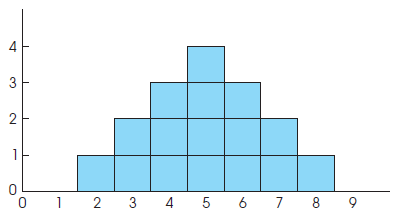
\includegraphics[width = 0.7\textwidth]{./cap6}
					\end{figure}
\end{frame}
\begin{frame}
	\begin{itemize}
		\justifying
		\item Dos caracterízticas se destacan del histograma de la distribución muestral de medias:
		\begin{enumerate}
			\justifying
			\item Las medias muestrales se mueven alrededor de la media.
			\item La distribución muestral de medias se aproxima a una curva normal.
		\end{enumerate}
		\item Finalmente, se puede usar la distribución muestral para responder preguntas de probabilidad relacionadas a las medias muestrales.
		\item Por ejemplo, si tomamos una muestra $n=2$ de la población original, ¿cuál es la probabilidad de obtener una media muestral mayor a 7?
	\end{itemize}
\end{frame}

\begin{frame}{Teorema del Límite Central}
	\begin{itemize}
		\justifying
		\item En situaciones más reales, con poblaciones y muestras mucho más grandes, el número de muestras posibles aumenta drásticamente.
		\item Por lo tanto, es imposible tener cada muestra posible.
		\item A pesar de esto, el teorema del límite central provee una descripción precisa de la distribución resultante si se seleccionan todas las muestras posibles.
	\end{itemize}
	\begin{block}{Teorema del Límite Central}
		Para cualquier población con media $\mu$ y desviación estándar $\sigma$, la distribución muestral de medias para un tamaño de muestra $n$ tendrá una media igual a $\mu$ y una desviación estándar de $\dfrac{\sigma}{\sqrt{n}}$. Además, se aproximará a una normal a medida que $n$ tiende a infinito.
	\end{block}
\end{frame}

\begin{frame}
\begin{itemize}
\justifying
\item El valor de este teorema recae en dos hechos:
\begin{enumerate}
	\justifying
	\item Describe la distribución muestral de medias para \emph{cualquier población}, sin importar su forma, media o desviación estándar.
	\item La distribución muestral de medias 	se aproxima a una normal de manera rápida. Cuando la muestra alcanza un $n=30$, la distribución es muy cercana a una normal.
\end{enumerate}
\item En resumen, el teorema del límite central identifica las tres caracterízticas básicas de una distribución: 
\begin{enumerate}[I]
\item Forma $\rightarrow$ Normal (Si la distribución poblacional es normal o si $n>30$)
\item Tendencia central $\rightarrow$ $\mu$
\item Dispersión $\rightarrow$ $\dfrac{\sigma}{\sqrt{n}}$
\end{enumerate}
\end{itemize}
\end{frame}

\begin{frame}
					\begin{figure}[H]
						\centering  
						\caption{} 
						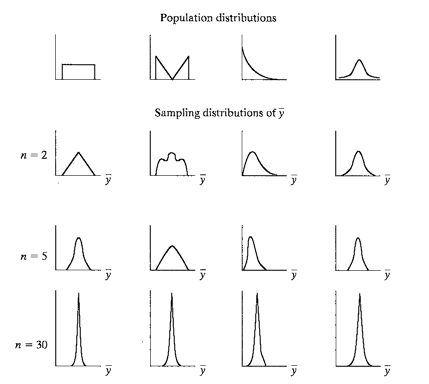
\includegraphics[width = 0.7\textwidth]{./cap5}
					\end{figure}
\end{frame}

\begin{frame}{Error Estándar}
\begin{itemize}
\justifying
\item La desviación estándar de una distribución muestral de medias se denomina \emph{error estándar} y se identifica con el símbolo $\sigma_{\bar{X}}$.
\item El error estándar cumple los dos propósitos de una desviación estándar:
\begin{enumerate}
\item Describe la distribución al decir si las medias muestrales están agrupadas o se dispersan a lo largo de un intervalo amplio.
\item Mide qué tan bien a una media muestral representa a toda la distribución de medias.
\end{enumerate}
\item Por tanto, un error estándar muy grande significa que existen grandes diferencias entre las muestras.
\item Dado que la media de la distribución es $\mu$, el error estándar provee un estimado de la distancia entre una media muestral $\bar{X}$ y la media poblacional $\mu$.
\end{itemize}
\end{frame}

\begin{frame}{Tamaño de la Muestra}
\begin{itemize}
\justifying
\item El tamaño de la muestra influencia la precisión con la cual la muestra representa la población.
\item Específicamente, una muestra grande es más precisa que una muestra pequeña.
\item En general, a medida que el tamaño de muestra aumenta, el error entre la media muestral y la media poblacional decrece.
\end{itemize}
\begin{block}{Ley de los Grandes Números}
A medida que el tamaño de muestra $n$ aumenta, es más probable que la media muestral sea cercana a la media poblacional.
\end{block}
$$\bar{X}\rightarrow \mu \quad sii \quad n\rightarrow \infty$$
\end{frame}

\begin{frame}{La Desviación Estándar Poblacional}
\begin{itemize}
\justifying
\item Ya se mencionó que existe una relación inversa entre el tamaño de muestra y el error.
\item El caso más extremo es la muestra que consiste de un sólo valor $n=1$.
\item En este caso, cada muestra es un valor único y la distribución muestral es idéntica a la distribución poblacional.
\item La desviación estándar de la distribución muestral, la cual es el error estándar, es la misma desviación estándar de la distribución poblacional.
\end{itemize}
$$Si \quad n=1 \rightarrow \sigma_{\bar{X}}=\dfrac{\sigma}{1}=\sigma$$
\end{frame}

\begin{frame}
	\begin{itemize}
\justifying
\item Para una distribución poblacional con $\sigma=10$, el error estándar varía de la siguiente manera según el tamaño de muestra:
	\end{itemize}
	\begin{figure}[H]
		\centering  
		\caption{} 
		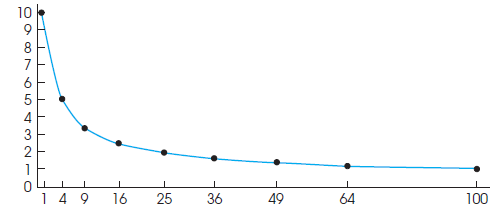
\includegraphics[width = 0.8\textwidth]{./cap1}
	\end{figure}
\end{frame}

\begin{frame}{Tres Distribuciones Distintas}
	\begin{columns}
		\begin{column}{.49\textwidth}
			\centering
			\only<1>{}\\[1ex]
	\begin{figure}[H]
		\centering  
		\caption{} 
		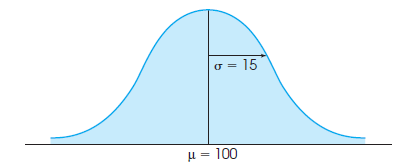
\includegraphics[width = 0.8\textwidth]{./cap2}
	\end{figure}
		\end{column}
		
		\begin{column}{.49\textwidth}
			\centering
			\only<1>{}\\[1ex]
	\begin{figure}[H]
		\centering  
		\caption{} 
		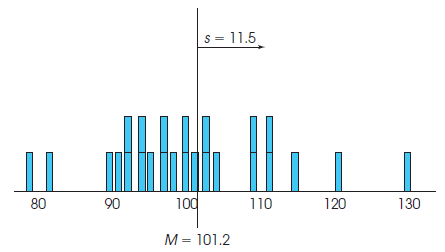
\includegraphics[width = 0.8\textwidth]{./cap3}
	\end{figure}
			
		\end{column}
					\end{columns}
					\begin{figure}[H]
						\centering  
						\caption{} 
						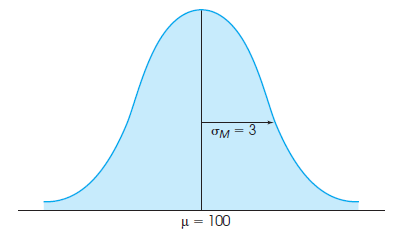
\includegraphics[width = 0.4\textwidth]{./cap4}
					\end{figure}

\end{frame}

\begin{frame}{Distribuciones muestrales para variables nominales}
\begin{itemize}
\justifying
\item Hasta el momento hemos considero variables continuas debido a que las variables nominales no se distribuyen normal.
\item Por ejemplo, la proporción de solteros en una población o la proporción de personas que votan por un partido en particular.
\item Asumamos que para el último censo, 32\% de la población colombiana es soltera. Es decir, 100-32=68\% de los colombianos no son solteros.
\item Bajo esta situación, si tomamos 10000 muestras de 300 colombianos, la proporción de solteros debe estar alrededor de 0.32
\end{itemize}
\end{frame}

\begin{frame}
\begin{itemize}
\justifying 
\item Denotemos la proporción poblacional de éxito como $P_U$. En este caso, $P_U=$ 0.32 es la proporción de solteros.
\item La letra $Q_U$ la usamos para nombrar a la proporción poblacional de fracasar. Para el ejemplo, $Q_U=1-P_U=$ 1$-$0.32=0.68 es la proporción de no ser soltero.
\item El error estándar se calcula de la siguiente manera:
$$\sigma_P=\sqrt{\dfrac{P_U*Q_U}{n}}=\sqrt{\dfrac{0.32*0.68}{300}}=0.026$$
\item Por lo tanto, la distribución muestral de la proporción de solteros en Colombia, tiene una media de 0.32 y una desviación estándar de 0.026
\end{itemize}
\end{frame}

\begin{frame}{Error de muestreo vs Error Estándar}
	\begin{itemize}
		\justifying
		\item El concepto general de error de muestreo es que una muestra usualmente no proporciona una representación perfecta de la población.
		\item De hecho, 50\% de las muestras tienen medias que son más pequeñas que $\mu$ (todo el lado izquierdo de la distribución). Similarmente,
		50\% de las muestras producen medias que sobreestiman la verdadera media de la población.
		\item Asumiendo que la distribución muestral es normal, para cada muestra se puede medir el error (o distancia) entre la media muestral y la media de la población.
		\item El \emph{error estándar} proporciona una manera de medir el ``promedio''  de la distancia entre una media muestral y la media poblacional. Es decir, el error estándar es una manera de medir el error de muestreo.
	\end{itemize}
\end{frame}
%%%%%%%%%%%%%%%%%%%%%%%%%%%%%%%%%%%%%%%%%%%%%%%%%%%%%%
\section{Probabilidad y Distribución Muestral}
\begin{frame}{Probabilidad y Distribución Muestral}
\begin{itemize}
\justifying
\item El principal uso de la distribución muestral de medias es encontrar la probabilidad asociada a cualquier muestra específica.
\item Recuerden que la probabilidad es equivalente a una proporción!
\item Dado a que la distribución muestral de medias presenta el conjunto de todas las posibles medias muestrales, podemos utilizar proporciones de esta distribución para determinar las probabilidades.
\item Además, gracias al teorema del límite central podemos utilizar la tabla de la distribución normal.
\end{itemize}
\end{frame}

\begin{frame}
\begin{itemize}
	\justifying
\item Asumamos que se realiza un examen a todos los estudiantes de la universidad. La media de la distribución es $\mu=$ 3.5 y la desviación estándar es $\sigma=$ 0.5. La distribución de la nota del examen es normal.
\item Si se toma una muestra de $n=25$ estudiantes, ¿cuál es la probabilidad que la media muestral sea mayor a $\bar{X}=$ 3.7?
\item ¿Qué sabemos?
\begin{enumerate}
\item La distribución muestral es normal porque la distribución del examen es normal.
\item La distribución muestral tiene una media de 3.5 dado que la media poblacional es $\mu=$ 3.5
\item La distribución muestral tiene una error estándar $\sigma_{\bar{X}}=$ 0.1
\end{enumerate}
$$\sigma_{\bar{X}}=\dfrac{\sigma}{\sqrt{n}}=\dfrac{0.5}{\sqrt{25}}=\dfrac{0.5}{5}=0.1$$
\end{itemize}
\end{frame}

\begin{frame}{La distribución muestral de medias}
	\begin{center}
		\scalebox{1}{
	\begin{tikzpicture}
	% define normal distribution function 'normaltwo'
	\def\normaltwo{\x,{4*1/exp(((\x-3)^2)/2)}}
	
	% input y parameter
	\def\x{4.5}
	\def\y{6}
	\def\z{3.01}
	% this line calculates f(y)
	\def\fx{4*1/exp(((\x-3)^2)/2)}
	\def\fy{4*1/exp(((\y-3)^2)/2)}
	\def\fz{4*1/exp(((\z-3)^2)/2)}
	% Shade orange area underneath curve.
	\fill [fill=green!60] (\x,0) -- plot[domain=\x:\y] (\normaltwo) -- ({\y},0) -- cycle;	
	% Draw and label normal distribution function
	\draw[color=blue,domain=0:6] plot (\normaltwo) node[right] {};
	
	% Add dashed line dropping down from normal.
	\draw[dashed] ({\x},{\fx}) -- ({\x},0) node[below] {3.7};
	\draw[dashed] ({\y},{\fy}) -- ({\y},0) node[below] {};
	\draw[dashed] ({\z},{\fz}) -- ({\z},0) node[below] {3.5};
	% Optional: Add axis labels
	\draw (-.2,2.5) node[left] {$f_x$};
	\draw (3,-.5) node[below] {$x$};
	
	% Optional: Add axes
	\draw[->] (0,0) -- (6.2,0) node[right] {};
	\draw[->] (0,0) -- (0,5) node[above] {};
	
	\end{tikzpicture}
		}
	\end{center}
	$$z=\dfrac{\bar{X}-\mu}{\sigma_{\bar{X}}}=\dfrac{3.7-3.5}{0.1}=\dfrac{0.2}{0.1}=2$$
\end{frame}

\begin{frame}
\begin{itemize}
\justifying
\item El z-score para una media muestral $\bar{X}=$ 3.5 será $z=+2$.
\item Por lo tanto, la probabilidad o proporción de encontrar una muestra con una media mayor a 3.7 es $p(z>2)=$ 0.0228=2.8\%.
\item Por lo tanto, es posible utilizar el z-score para describir la ubicación exacta de cualquier muestra específica  dentro de la distribución muestral de medias.
\item Considerando la misma distribución del ejemplo anterior, ahora encontremos el rango de valores que son esperados para la media muestral el 80\% de las veces. 
\item Ya sabemos que la distribución es normal con una media esperada de $\mu=$ 3.5 y desviación estándar $\sigma_{\bar{X}}=$ 0.1.
\end{itemize}
\end{frame}

\begin{frame}
\begin{itemize}
\justifying
\item Nuestro objetivo es encontrar el rango de valores límites del 80\% medio de la distribución.
\item Dado que la distribución es normal, podemos usar la tabla para encontrar los valores que dividen el 10\% a lado y lado de la distribución.
\item En la tabla encontramos que para una proporción o probabilidad de 0.9, el z-score es 1.28
\item De esta manera, los límites del 80\% medio de la distribución corresponden a $z=-$ 1.28 y $z=+$ 1.28
\end{itemize}
\end{frame}

\begin{frame}
\begin{itemize}
\justifying
\item Por definición, un z-score de 1.28 representa una ubicación que está a 1.28 desviaciones estándar de la media.
\item Con un error estándar de 0.1, la distancia a la media es de 1.28*0.1 $=$ 0.128
\item La media es $\mu=$ 3.5, por lo cual, una distancia de 0.128 en ambas direcciones produce un rango de valores entre 3.372 y 3.628
\item De esta manera, 80\% de todas las posibles medias muestrales se encuentran dentro de un intervalo entre 3.372 y 3.628
\item Otra interpretación es que si seleccionamos una muestra $n=25$, estamos 80\%  seguros que la media de la muestra va a encontrarse en ese intervalo.
\end{itemize}
\end{frame}

\section{Intervalos de Confianza}
\begin{frame}{Intervalos de Confianza}
\begin{itemize}
\justifying
\item Es claro que sólo en contadas ocasiones se tendrán los valores para la media y la desviación estándar poblacional.
\item Al trabajar con una de las posibles muestras, es necesario acercarnos a los parámetros poblacionales a partir de los estadísticos muestrales que se tienen disponibles.
\item Un {\bf intervalo de confianza} es un rango de valores posibles de un parámetro expresado en un grado o nivel específico de confianza.
\item Con los intervalos de confianza tomamos una estimación puntual de la muestra y la acoplamos con el conocimiento que tenemos sobre las distribuciones muestrales.
\item Con los intervalos de confianza proyectamos un rango conocido y calculable de error respecto a la estimación puntual. 
\end{itemize}
\end{frame}

\begin{frame}
\begin{itemize}
\justifying
\item Supongamos que tomamos una muestra de $n=300$ estudiantes de la universidad con un promedio de edad de $\bar{X}=$ 20.5 años y $s_{X}=$ 1.5.
\item Sabemos que la distribución muestral de medias toma forma de curva normal cuando $n>30$.
\item La edad promedio de la muestra debe estar cerca del parámetro poblacional real (la edad media de todos los estudiantes de la universidad).
\item Dado lo anterior, podemos decir con seguridad que el 95\% de las muestras caen dentro de casi 2 errores estándar del parámetro real (Regla 68-95-99).
\item Al calcular un intervalo de confianza, no trabajamos con muchas muestras ni calculamos áreas bajo la curva de distribución muestral. 
\end{itemize}
\end{frame}

\begin{frame}{Nivel de Confianza}
\begin{itemize}
\justifying
\item Por el contrario, trazamos una única muestra y calculamos una estimación puntual como la media. 
\item El {\bf nivel de confianza} nos dice nuestra tasa de éxito, es decir, con qué frecuencia el parámetro poblacional se encuentra en el rango del intervalo de confianza.
\item Usualmente, los grados de confianza más utilizados en las ciencias sociales son el 95 y 99\%.
\item Al confiar en una muestra, sabemos que podemos fallar en la predicción debido a la existencia del error de muestreo.
\end{itemize}
\end{frame}

\begin{frame}{Nivel de Significancia}
\begin{itemize}
\justifying

\item La única manera de tener total certeza sobre nuestras conclusiones es reunir datos de la población.
\item Cabe destacar que la cantidad de error es conocida. El nivel de error esperado es la diferencia entre el nivel de confianza y la ``confianza perfecta'' del 100\%.
\item En otras palabras, si estamos 95\% seguros acerca de nuestro resultado, estamos 5\% inseguros acerca de este.
\end{itemize}
$$Nivel \, de \, confianza =95\%$$
$$Nivel \, de \, significancia = \alpha= 100\%-95\%=5\%$$
\end{frame}


\begin{frame}
	\begin{itemize}
\item ¿A qué distancia del parámetro poblacional se encuentra nuestra media muestral para un nivel de confianza del 95\%?
\item A partir dela tabla de la normal podemos encontrar los valores Z críticos para el nivel de significancia $\alpha$ ($Z_{\alpha}$). 
\end{itemize}
	\begin{center}
		\scalebox{0.5}{
			\begin{tikzpicture}
			% define normal distribution function 'normaltwo'
			\def\normaltwo{\x,{4*1/exp(((\x-3)^2)/2)}}
			
			% input y parameter
			\def\x{0}
			\def\y{1}
			\def\w{5.02}
			\def\q{6}
			\def\z{3.01}
			
			
			% this line calculates f(y)
			\def\fx{4*1/exp(((\x-3)^2)/2)}
			\def\fy{4*1/exp(((\y-3)^2)/2)}
			\def\fz{4*1/exp(((\z-3)^2)/2)}
			\def\fw{4*1/exp(((\w-3)^2)/2)}
			\def\fq{4*1/exp(((\q-3)^2)/2)}
			% Shade orange area underneath curve.
			\fill [fill=orange!60] (\x,0) -- plot[domain=\x:\y] (\normaltwo) -- ({\y},0) -- cycle;
					\fill [fill=red!60] (\y,0) -- plot[domain=\y:\z] (\normaltwo) -- ({\z},0) -- cycle;
					\fill [fill=red!60] (\z,0) -- plot[domain=\z:\w] (\normaltwo) -- ({\w},0) -- cycle;
			\fill [fill=orange!60] (\w,0) -- plot[domain=\w:\q] (\normaltwo) -- ({\q},0) -- cycle;
			% Draw and label normal distribution function
			\draw[color=blue,domain=0:6] plot (\normaltwo) node[right] {};
			
			% Add dashed line dropping down from normal.
			\draw[dashed] ({\x},{\fx}) -- ({\x},0) node[below] {};
			\draw[dashed] ({\y},{\fy}) -- ({\y},0) node[below] {$-1.96$};
			\draw[dashed] ({\z},{\fz}) -- ({\z},0) node[below] {$0$};
			\draw[dashed] ({\w},{\fw}) -- ({\w},0) node[below] {$1.96$};
			\draw[dashed] ({\q},{\fq}) -- ({\q},0) node[below] {};
			% Optional: Add axis labels
			\draw (-.2,2.5) node[left] {$f_x$};
			\draw (3,-.5) node[below] {$x$};
			
			% Optional: Add axes
			\draw[->] (0,0) -- (6.2,0) node[right] {};
			\draw[->] (0,0) -- (0,5) node[above] {};
			
			\end{tikzpicture}
		}
	\end{center}
\begin{itemize}
\justifying
\item El área roja representa el 95\% de las medias muestrales, mientras que, las dos áreas naranjas representan el 5\% de las medias que están fuera de los dos valores críticos.
\item 95\% de las observaciones de una normal están dentro de 1.96 SD.
\end{itemize}
\end{frame}

\begin{frame}{Margen/Término de Error}
\begin{itemize}
\justifying
\item Ya sabemos que el $Z_{\alpha}=$ 1.96 y que $s_X=1.5$. Por lo tanto:

$$\sigma_{\bar{X}}=\dfrac{1.5}{\sqrt{300}}=\dfrac{1.5}{17.3}=0.08$$
\item El margen de error será igual a $Z_{\alpha}*\sigma_{\bar{X}}=0.08*1.96=0.169$
\item El intervalo de confianza estará entre:
$$IC\, de\, 95\%\, de\, \mu=\bar{X}\pm (Z_{\alpha})(\sigma_{\bar{X}})$$
\begin{center}
Límite Inferior = 20.5 $-$ 0.169 = 20.3 \\
Límite Superior = 20.5 $+$ 0.169 = 20.6  
\end{center}
\end{itemize}
\end{frame}

\begin{frame}{¿Cuál es la interpretación?}
\begin{itemize}
\justifying
\item Estoy 95\% seguro de que la edad promedio de los estudiantes de la universidad se ubica entre 20.3 y 20.6 años.
\item En otras palabras, si se realizan los mismos procedimientos muestrales 100 veces, el parámetro poblacional $\mu$ estará entre los intervalos calculados el 95 de esas veces.
\end{itemize}

\end{frame}

\begin{frame}
					\begin{figure}[H]
						\centering  
						\caption{} 
						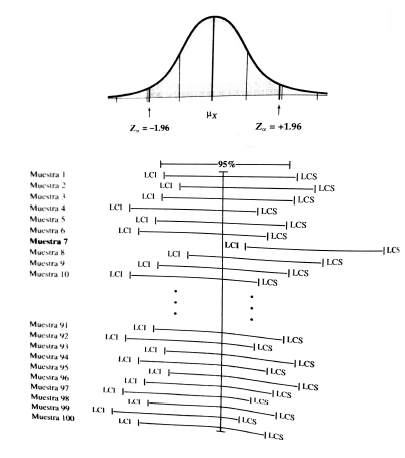
\includegraphics[width = 0.6\textwidth]{./cap7}
					\end{figure}
\end{frame}

\begin{frame}{Grado de Precisión}
\begin{itemize}
\justifying
\item Entre mayor sea el nivel de confianza estipulado, mayor será el margen de error y por lo tanto será menos preciso el intervalo de confianza.

$$ Z_{0.05}=1.96 \quad vs \quad Z_{0.01}=2.58$$

\item Entre mayor sea el tamaño de la muestra, más preciso será el intervalo de confianza.

$$\sigma_{\bar{X}}=\dfrac{s_X}{\sqrt{n}}\, entonces \, si\, \uparrow n \rightarrow \downarrow \sigma_{\bar{X}}  $$
\end{itemize}
\end{frame}
\end{document}